\section{Accepttest}
Indgangsimpedansen for alle indgange gav samme resultat ved målingerne. Indgangsimpedansen, for et slukket og et tændt signal, er, som vist i Appendiks \ref{maalejournal_indgangsvaelger}, henholdsvis 22,62 k\ohm~ og 31,56 k\ohm . Da disse begge er over 22 k\ohm~samt stemmer overens med beregningerne, indenfor komponenttolerancerne, er indgangsimpedansen acceptabel.

Frekvensgangen for 200 mV og 2 V inputspænding, er meget éns, derfor tages der kun udgangspunkt i den ene. Det er valgt at konkludere på frekvensgangen for 200 mV, da denne giver det største udsving. En graf over de målte data kan ses på figur \ref{fig:indacc:frek200mv}.
\begin{figure}[h]
\centering
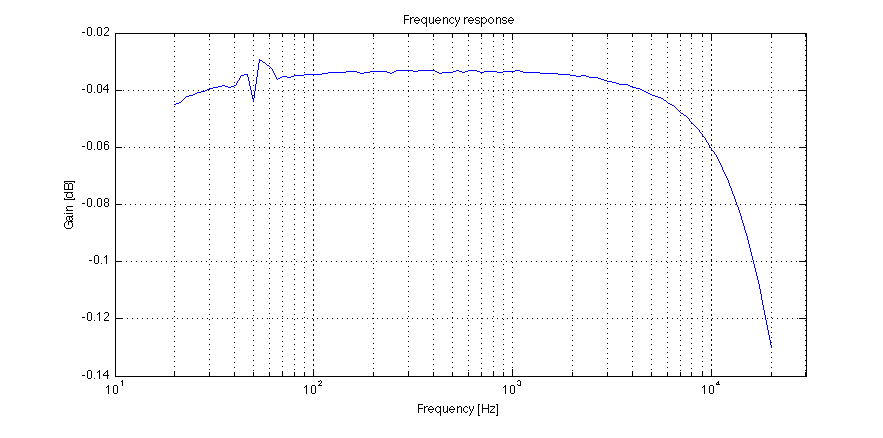
\includegraphics[width=\textwidth]{maalerapporter/indgangsvaelger/Indgangsvlger-mic-200mv-frek.png}
\caption{Målt frekvensgang for mikrofonindgangen på indgangsvælgeren ved 200 mV inputspænding}
\label{fig:indacc:frek200mv}
\end{figure}

Dæmpningen af et tændt signal ved referencefrekvensen, 1 kHz, er i målingen aflæst til 0,034 dB. Den frekvens som afviger mest fra denne værdi er ved 20 kHz, som aflæses til en dæmpning på 0,13 dB. Dette giver en afvigelse på ca. 0,1 dB, hvilket er meget tæt på det simulerede og under det opstillede krav på 0,375 dB. Dette er derfor acceptabelt.

Målingerne viser, på figur \ref{fig:indaccept:slukketmaaling}, at dæmpning ved 1 kHz er på ca. 114 dB. Denne dæmpning er større end det opstillede krav på 50 dB og er derfor accepteret.
\begin{figure}[h]
\centering
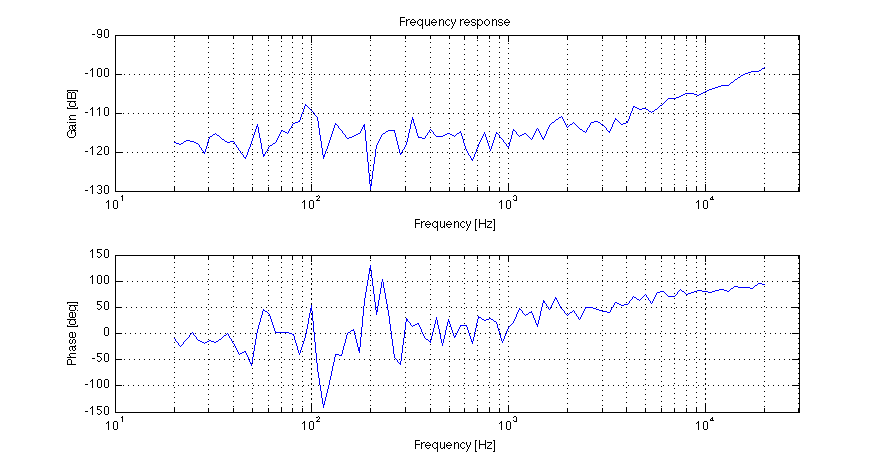
\includegraphics[width=\textwidth]{maalerapporter/indgangsvaelger/Indgangsvlger-mic-2v-slukket-frek.png}
\caption{Frekvensgangen og fasedrejet for mikrofonindgangen for et slukket signal, på indgangsvælgeren ved 2 V. Disse målinger er sandsynligvis støj, da spændingerne er på et meget lavt niveau}
\label{fig:indaccept:slukketmaaling}
\end{figure}	

THD simuleres til 0,062 \% ved en peakspænding på 2 V, ved 1 kHz. Ved en THD måling, illustreret på figur \ref{fig:accind:thd2v}, aflæses THD'en ved 1 kHz til 0,1 \%. 
\begin{figure}[h]
\centering
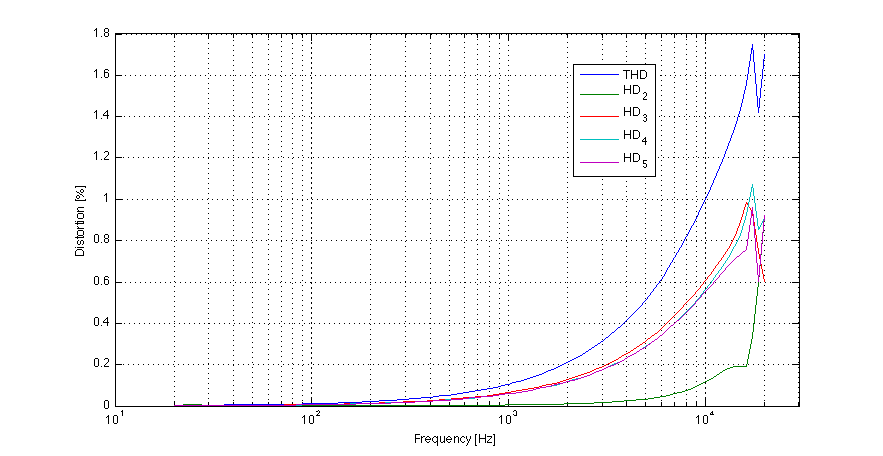
\includegraphics[width=\textwidth]{maalerapporter/indgangsvaelger/Indgangsvlger-mic-2v-thd.png}
\caption{Målt THD for mikrofonindgangen på indgangsvælgeren ved 2 V inputspænding}
\label{fig:accind:thd2v}
\end{figure}
Det kan dog konkluderes at THD ikke er lav nok. Dette kan delvist løses ved at benytte en anden operationsforstærker, f.eks. OPA27 i stedet for LM324. Det er dog tydeligt, ud fra Appendiks F, at transistorerne ikke afbryder helt, når signalet ikke skal slukkes og at de derfor har en indflydelse. Dette er ikke optimalt og det ville derfor være bedre at benytte en transistor, som afkobler bedre i slukket tilstand.

\begin{table}[h]
\centering
\begin{tabular}{l|r|r}
\hline\hline
Område & Krav & Status \\
\hline\hline
Antal trin i & 4 & \checkmark \\
indgangsvælgeren & \\[4pt]
Indgangsimpedans & > 22 k\ohm & \checkmark \\[4pt]
Frekvensgang & $\pm$ 0,375 dB ved 20 Hz - 20 kHz, ref. 1 kHz & \checkmark \\
& $\pm$ 0,75 dB fra 20 Hz til 63 Hz & \checkmark\\
& $\pm$ 0,75 dB fra 12,5 kHz til 20 kHz & \checkmark\\[4pt]
Dæmpning af slukket & > 50 dB ved 1 kHz & \checkmark \\
indgangssignal & \\
\hline\hline
\end{tabular}
\caption{Oversigt over status af krav til indgangsvælgeren}
\label{tab:krav_indgangsvaelger}
\end{table}